\documentclass[11pt,oneside]{book}
\pagestyle{plain}
\usepackage{graphicx}
\usepackage{makeidx}
\usepackage{nomencl}
\usepackage{listings}
\usepackage{multirow}
\usepackage{float}

\textheight=235mm
\textwidth=145mm
\topmargin=0mm
\headheight=0mm
\headsep=0mm

% Spacing between rows
\renewcommand{\arraystretch}{1.3}

% These must be changed for double sided output !
\usepackage{geometry}
\geometry{margin=2.5cm}

% Custom commands
\newcommand{\mychapter}[2]{
    \setcounter{chapter}{#1}
    \setcounter{section}{0}
    \chapter*{#2}
    \addcontentsline{toc}{chapter}{#2}
}

\makeindex
\makeglossary
\begin{document}

% set line spacing to 1.5B
\baselineskip = 17pt
\title{
    \centerline{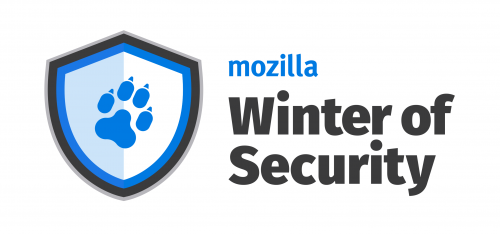
\includegraphics[height=40mm]{./MWOS.png}}
Multifactor Authentication and Session Resumption in OpenVPN}
\author{
    Report submitted in accordance with the requirements of \\
    the Indian Institute of Technology, Kanpur \\
    by \\
    Harshwardhan Sharma (11299),\\
    Shivanshu Agarwal (11688),\\
    Srijan R. Shetty (11727)
}
\date{November 2014}
\maketitle
\frontmatter

\mychapter{0}{Abstract}
Mozilla uses OpenVPN with MFA via deferred C plugins and pythons scripts.
However, there are several caveats that require non-plugin based modifications,
such as One Time Passwords (OTP) client input and session tracking.
The goal of this project has been to research and provide a first class user experience
to the end user when using MFA with OpenVPN; including the support for session resumption
and backwards compatibility with older versions of OpenVPN.
In the long run, the authors would want their implementation of the changes discussed below
be merged with the upstream version of OpenVPN.


% Contents not put in table of contents by default so add it separately
\tableofcontents
\addcontentsline{toc}{chapter}{Contents}

\mychapter{0}{Acknowledgement}
The authors would like to thank Professor Dheeraj Sanghi for his continued guidance
and support, Guillaume Destuynder of Mozilla who mentored the authors despite his
hectic schedule and lastly Mozilla for giving the authors an opportunity to work on
a project like OpenVPN under its aegis.\\
The authors wish to thank the University of Liverpool Computing Services Department
for the development of this \LaTeX \ thesis template.

% Create glossary and add
\printglossary
\addcontentsline{toc}{chapter}{Nomenclature}

\mainmatter

\mychapter{1}{OpenVPN}
\section{Introduction}
A Virtual Private network allows two devices to securely communicate with each other
over a possibly insecure public network. This concept when extended to networks
allows for secure communications between different private networks over an
insecure network (most often the internet), through tunnelling and there by allowing
all these private networks to be virtually connected.

OpenVPN \footnote{http://openvpn.net} is a GNU General Public
Licensed \footnote{http://www.gnu.org/copyleft/gpl.html} implementation of a
Virtual Private Network written in C maintained by the OpenVPN project.
The source of OpenVPN is freely available for modification; thereby encouraging willing
developers to contribute to the development of OpenVPN. The changes made, if accepted
by the developer community are eventually merged with the upstream version of OpenVPN.

\section{Architecture}
\subsection{Encryption}
OpenVPN can use either of OpenSSL or PolarSSL for encryption and decryption. The choice of the SSL
library can be provided during compilation of OpenVPN binary.

\subsection{Authentication Modes}
OpenVPN provides for two authentication modes:

\begin{enumerate}
    \item {Static Key}: In this mode, a key is generated and shared between the users before
        the establishment of a tunnel. The static key comprises of four independent keys: HMAC send,
        HMAC receive, encrypt key and decrypt key.
    \item {TLS}: In this mode, a bidirectional session using certificates is established between.
        On a successful TLS/SSL authentication, both side exchange source material for the key
        which is used to generate eight different keys (for the client and server). The key
        generation depends on the key method provided. Key method 1 derives it's source material
        from OpenSSL RAND\_bytes while key method 2 derives it from TLS PRF\cite{RFC5246} function.
        Refer to \
\end{enumerate}

\subsection{Key Methods}
The current architecture of OpenVPN supports two key methods:

\begin{enumerate}
    \item \emph{Key Method 1}, the legacy key method only checks for the validity of certificates.
        Refer to Appendix \ref{OpenVPN:Protocol} on page \pageref{OpenVPN:Protocol} for details.
    \item \emph{Key Method 2}, in addition to checking for the validity of certificates, allows for
        authentication of the user through username and password. The verification of username and
        password is delegated to either a script or a plugin which returns a binary result
        indicating a success or failure.
        Refer to Appendix \ref{OpenVPN:Protocol} on page \pageref{OpenVPN:Protocol} for details.
\end{enumerate}


\subsection{Networking}
TLS/SSL protocol mandates a reliable transport layer, while on the other hand the tunnelled IP
packets require a unreliable layer beneath them. To overcome this reliability-layer collision,
OpenVPN multiplexes both these connections.
The SSL/TLS session used for authentication and key exchange is still sent over UDP but with a
reliability layer provided by OpenVPN. Multiplexed with SSL/TLS session are the IP packets, which
after being encrypted and signed by and HMAC are directly passed over the UDP layer. This ensures
that each of these channels gets what it expects from the layer beneath it. Additionally, both these
channels are completely independent of each other and hence do not interfere with each other's
functioning.\\

\begin{figure}[h]
    \begin{verbatim}
        SSL/TLS -> Reliability Layer -> \
                   --tls-auth HMAC       \
                                          \
                                           > Multiplexer ----> UDP
                                          /                    Transport
        IP        Encrypt and HMAC       /
        Tunnel -> using OpenSSL EVP --> /
        Packets   interface.
    \end{verbatim}
    \vspace{-6mm}
    \caption{OpenVPN Networking}
\end{figure}

Note: In recent releases OpenVPN, support TCP as a transport layer as well.

\section{Protocol}
OpenVPN uses a custom protocol\cite{OpenVPN_Security} for communications which is attached in appendix
\ref{OpenVPN:Protocol} on page \pageref{OpenVPN:Protocol} for perusal.

\mychapter{2}{Multifactor Authentication}
\section{Introduction}
\label{MFA:Introduction}
Multifactor Authentication, henceforth used interchangeably with MFA, hardens access control
by challenging a user on at least two out of the following three factors of authentication.

\begin{enumerate}
    \item \emph{Knowledge Factor}: The knowledge factor of authentication comprises of
        authentication methods which tests the user for the knowledge of a pre-shared secret.
        \emph{"things only the user knows"}. For example: ATM Pins, website passwords.
    \item \emph{Possession Factor}: The possession factor of authentication comprises of
        authentication methods which tests the user for the possession of an entity.
        \emph{"things only the user has"}. For example: Smart cards, ATM Cards.
    \item \emph{Inherence Factor}: The inherence factor of authentication comprises of
        authentication methods which tests the user for possession of \emph{"things only
        the user is"}. For example: Retinal scans, Fingerprint scans.
\end{enumerate}

While conventional methods of authentication only take into account a knowledge factor,
(most internet websites which a username password mechanism to authenticate users)
multi factor authentication includes at least two different factors from the aforementioned
list and might even have multiple authentication methods for a particular factor.

\section{Challenges}
\begin{enumerate}
    \item \textbf{Singled Threaded}: OpenVPN is single threaded process with an event loop which
        allows it to handle concurrent connection requests. Every request fires a timer in OpenVPN
        and if authentication does not succeed before the time quantum expires, the connection is
        reset. The time-out being tried and tested, was not up for modification.
        Considering that current MFA schemes like OTP depend upon non-reliable mechanisms like
        SMS during which the time-out might expire, we made use of the plugin system of OpenVPN
        which allowed for deferred authentication. Hence overcoming the hurdle of time-out
        during authentication.
        (Refer to \ref{MFA:Mechanism} on page \pageref{MFA:Mechanism} for implementation details.)
    \item \textbf{MFA Types}: Multiple solutions are available for multifactor authentication, hence
        there was a need to provide an extensible mechanism to use the different available MFA
        authentication schemes. (Refer to \ref{MFA:Types} on page \pageref{MFA:Types} for
        implementation details.)
    \item \textbf{Backwards Compatibility}: Considering that not all servers will want to support
        MFA, all the changes were introduced in a non breaking fashion.
        (Refer to \ref{MFA:BackwardCompat} on page \pageref{MFA:BackwardCompat} for implementation details.)
    \item \textbf{Defensive Coding}: OpenVPN uses a defensive style of coding by using various
        abstractions for garbage collection, memory allocation to overcome the shortcomings of C.
\end{enumerate}

\section{Implementation}
\begin{figure}[t]
    \label{MFA:Old Packet}
    \begin{verbatim}
            +-------------------------------------------------------+
            |    TLS plaintext packet (if key_method == 2):         |
            +-------------------------------------------------------+
            |  Literal 0 (4 bytes).                                 |
            |  key_method type (1 byte).                            |
            |  key_source structure (pre_master only                |
            |      defined for client -> server).                   |
            |  options_string_length, including null (2 bytes).     |
            |  Options string (n bytes, null terminated,            |
            |          client/server options string must match).    |
            |                                                       |
            |  [The username/password data below is optional]       |
            |  username_string_length, including null (2 bytes).    |
            |  Username string (n bytes, null terminated).          |
            |  password_string_length, including null (2 bytes)     |
            |  Password string (n bytes, null terminated).          |
            +-------------------------------------------------------+
    \end{verbatim}
    \vspace{-10mm}
    \caption{Old Plaintext packet structure}
\end{figure}

\label{MFA:Implementation}
\subsection{Packet Structure}
The packet structure of key method 2 - Refer to \ref{MFA:Old Packet} on page \pageref{MFA:Old Packet} -
was augmented with the addition of a MFA-username and a MFA-password in the options of TLS plaintext
packet (key method 2) - Refer to \ref{MFA:New Packet} on page \pageref{MFA:New Packet} -
following username and password fields for AUTH-USERPASS. To ensure backwards
compatibility, all augmentations were made at the end of the packet.

\begin{figure}[t]
    \label{MFA:New Packet}
    \centering
    \begin{verbatim}
            +-------------------------------------------------------+
            |    TLS plaintext packet (if key_method == 2):         |
            +-------------------------------------------------------+
            |  Literal 0 (4 bytes).                                 |
            |  key_method type (1 byte).                            |
            |  key_source structure (pre_master only                |
            |      defined for client -> server).                   |
            |  options_string_length, including null (2 bytes).     |
            |  Options string (n bytes, null terminated,            |
            |          client/server options string must match).    |
            |                                                       |
            |  [The username/password data below is optional]       |
            |  username_string_length, including null (2 bytes).    |
            |  Username string (n bytes, null terminated).          |
            |  password_string_length, including null (2 bytes)     |
            |  Password string (n bytes, null terminated).          |
            |                                                       |
            |  [The MFA data below is optional]                     |
            |  mfa_username_string_length, including null (2 bytes).|
            |  MFA Username string (n bytes, null terminated).      |
            |  mfa_password_string_length, including null (2 bytes) |
            |  MFA Password string (n bytes, null terminated).      |
            +-------------------------------------------------------+
    \end{verbatim}
    \vspace{-10mm}
    \caption{New plaintext packet structure}
\end{figure}

\subsection{MFA Plugin Types}
\label{MFA:Types}
Three new OpenVPN plugin types have been introduced to support MFA.

\subsubsection{MFA types}
\begin{itemize}
    \item \textbf{OPENVPN\_PLUGIN\_AUTH\_MFA\_OTP\_VERIFY} \\
        A one time password - \emph{OTP}\footnote{OTPs are a suite of digits, usually 6 to 8 digits
        long, which work only once and are invalidated after use (HOTP\cite{HOTP}) or valid for a
    certain period of time (TOTP\cite{TOTP})} - consist of only a password which can be conveniently
        delivered to the user using SMS, an OTP-stick, or an application like Google Authenticator.
    \item \textbf{OPENVPN\_PLUGIN\_AUTH\_MFA\_USER\_PASS\_VERIFY} \\
        The conventional username-password scheme requires the user to provide
        both a username and password for multifactor authentication.
    \item \textbf{OPENVPN\_PLUGIN\_AUTH\_MFA\_PUSH\_VERIFY} \\
        No input is required by the user in a push message\footnote{A push message is a push
        notification to a device owned by the user. On accepting the push message, the device
        sends the response to the server which in turn relays it to the OpenVPN plugin} except
        the confirmation of a push from a pre selected device.
\end{itemize}

In case of OTP authentication, the username field is set to the Common Name of the user and the OTP
is sent as the password. The Common Name is sent as the username in PUSH with an empty string as
password. The username and password fields are populated with the user supplied values in case of
USER-PASS.

To allow for maximum extensibility of MFA, the actual implementation of each kind of of MFA
is left to the plugin/script writer to prevent a vendor lock down.

\subsection{Authentication mechanism}
\label{MFA:Mechanism}
At the time of booting, the plugin/script mentioned in the configuration file is registered
by OpenVPN's plugin system (only one plugin/script is allowed). During authentication, OpenVPN
simply calls the registered plugin/script waits for a success/failure response. On receiving a
success, OpenVPN continues on with the rest of the protocol; and on receiving a failure, OpenVPN
immediately terminates the client connection by sending the client a \emph{SIGTERM} signal.

\subsection{Backwards Compatibility}
The following scenarios have been addressed under the backwards compatibility flag:\\

{
    \centering
    \begin{tabular}{|c|c|c|c|}
        \hline
        \textbf{Compatibility} & \textbf{Server} & \textbf{Client} & \textbf{Action} \\

        \hline
        \multirow{3}{*}{Enabled} & \multirow{3}{*}{New Server, MFA-enabled} & New Client, MFA-Enabled & MFA-auth\\
                                 & & New Client, MFA-Disabled & auth-failure\\
                                 & & Old Client & old-auth\\
        \hline
        Disabled & New Server, MFA-enabled & Old Client & auth-failure\\

        \hline
        \multirow{2}{*}{*} & \multirow{2}{*}{New Server, MFA-disabled} & New Client, MFA-Enabled & MFA-auth\\
                           & & New Client, MFA-disabled & old-auth\\
        \hline
        * & New Server, MFA-disabled & Old Client & old-auth\\
        \hline
        \multirow{2}{*}{*} & \multirow{2}{*}{Old Server} & New Client, MFA-Enabled & MFA-auth\\
                           & & New Client, MFA-Disabled & MFA-auth\\
        \hline
    \end{tabular}
}

\section{Configuration}
\subsection{Server}
To enable multifactor authentication in the server using a script, the following line needs to be
included in the configuration file of the server:

\begin{verbatim}
    mfa-method [method-type] [script file name] [via-env/via-file]
\end{verbatim}

\noindent Here method-type is one of 'otp', 'push' or 'user-pass'. For example:
\begin{verbatim}
    mfa-method otp auth.pl via-file
\end{verbatim}

\noindent Multifactor authentication can also be enabled using plugins, the incantation for the same is:
\begin{verbatim}
    mfa-method [method-type]
    plugin [plugin shared object file]
\end{verbatim}

\subsection{Client}
To enable multifactor authentication in the client, the following line needs to be included in the
configuration file of the client:

\begin{verbatim}
    mfa-method [method-type]
\end{verbatim}

\subsection{Backwards Compatibility}
\label{MFA:BackwardCompat}
The server can allow connections from old clients during the initial transition phase by adding
the following line to its configuration file:

\begin{verbatim}
    mfa-backward-compat
\end{verbatim}

\section{Future Work}
\begin{itemize}
    \item \textbf{Session Resumption}: Most web based MFA schemes allow for session resumption,
        wherein MFA authentication is bypassed if the client has authenticated itself within
        a specified time period.
\end{itemize}

\section{Release Notes}
\begin{enumerate}
    \item OpenVPN should be compiled with the enable-mfa (enabled by default) flag for Multifactor
        Authentication support.
    \item The changes introduced by Multifactor Authentication despite being a complete overhaul of key method
          2 constitute only a minor patch according to the Semver specification. \footnote{Semver or Semantic
          Versioning is a system of naming software releases as MAJOR.MINOR.PATCH. A major change introduces
          breaking changes to software. A minor change introduces non breaking features to software.
          A patch introduces non breaking fixes to the software.}
\end{enumerate}

\section{Commit Log}
Refer to Appendix \ref{MFA:Commit} on page \pageref{MFA:Commit} for the commit log.

\mychapter{3}{Session Resumption}
\section{Introduction}
Multifactor Authentication trades security to convenience. While addition factors of authentication
reduces the probability of the impersonation of user even in the face of the loss of password,
they increase the complexity of authentication and ergo lead to a bad user experience.
To provide a smoother user experience, most web based multifactor authentication
flows provide for session resumption. Session resumption allows devices which on which the user has authenticated
once using multifactor authentication to transparently store an additional secret --- the session
token --- between the client and the server. The session token expires after a certain period of
time, and provides for the additional factor of authentication without taking recourse to MFA.

\section{Challenges}
\textbf{TODO}

\section{Implementation}
The chosen method of session resumption makes use of session tickets/tokens and not TLS session
resumption owing to the wide variety of attacks\cite{TLS_Insecure} demonstrated on the lesser used TLS features.

\section{Current Architecture}
OpenVPN currently has no provision for session resumption, the entire scaffolding for session
resumption was built on the Multifactor Authentication. \footnote{ Refer to \ref{MFA:Implementation}
on page \pageref{MFA:Implementation} for details}.

\section{Configuration}
Session Resumption, builds upon Multifactor Authentication, hence configuration parameters of MFA
need to be setup for any of the following configuration parameters to have effect.

\subsection{Server}
To enable session resumption in the server, a token expiration time must be provided in the server
configuration file.

\begin{verbatim}
    mfa-session-expiration [session-validity (in hours)]
\end{verbatim}

\subsection{Client}
To enable multifactor authentication in the client, a file to store session tokens must be provided
in the client configuration file.

\begin{verbatim}
    mfa-session-file [filename]
\end{verbatim}

\noindent
In the absence the above configuration parameter, the user is warned and session resumption is
disabled.

\section{Future Work}
\textbf{TODO}

\section{Release Notes}
\textbf{TODO}

\section{Commit Log}
Refer to Appendix \ref{Session:Commit} on page \pageref{Session:Commit} for the commit log.

\appendix
\chapter{OpenVPN Protocol}
\cite{OpenVPN_Security}
\label{OpenVPN:Protocol}
\lstinputlisting{protocol.c}

\chapter{Multifactor Authentication}
\label{MFA:Commit}
\section{Commit Log}
Taken form \emph{https://github.com/harsh1618/openvpn/commits/feature/mfa}.\\
\lstinputlisting{mfa-commit-log}

\chapter{Session Resumption}
\label{Session:Commit}
\section{Commit Log}
Taken form \emph{https://github.com/harsh1618/openvpn/commits/feature/session}.\\
\lstinputlisting{session-commit-log}

\bibliographystyle{plain}
\bibliography{thesis}
\addcontentsline{toc}{chapter}{Bibliography}

\printindex
\addcontentsline{toc}{chapter}{Index}

\end{document}
